%%%%%%%%%%%%%%%%%%%%%%%%%%%%%%% beamer %%%%%%%%%%%%%%%%%%%%%%%%%%%%%%%%%%%%%%%%%%%%%%%%%
% To run - pdflatex filename.tex
%	   acroread filename.pdf
%%%%%%%%%%%%%%%%%%%%%%%%%%%%%%%%%%%%%%%%%%%%%%%%%%%%%%%%%%%%%%%%%%%%%%%%%%%%%%%%%%%%%%%%
%\documentclass[handout,compress,gray]{beamer}
\RequirePackage{flashmovie}
\documentclass[utf8x,compress,black]{beamer} 
\mode<presentation>
\usetheme{Madrid}

\hypersetup{pdfpagemode=FullScreen}%makes your presentation go automatically to full screen

\usepackage[absolute,overlay]{textpos}
\setlength{\TPHorizModule}{1mm}
\setlength{\TPVertModule}{1mm}

\usepackage{silence}

\usepackage{scalerel,stackengine}
\def\apeqA{\SavedStyle\sim}
\def\apeq{\setstackgap{L}{\dimexpr.5pt+1.5\LMpt}\ensurestackMath{%
  \ThisStyle{\mathrel{\Centerstack{{\apeqA} {\apeqA} {\apeqA}}}}}}



\definecolor{Red}{rgb}{1,0,0}
\xdefinecolor{olive}{cmyk}{0.64,0,0.95,0.4}
\useoutertheme[subsection=false]{smoothbars}
\beamertemplateshadingbackground{red!9}{blue!4}

\usepackage{subfigure}
%\usepackage{natbib}
%\usepackage{biblatex}
%\usepackage[backend=bibtex]{biblatex}
\usepackage{natbib}
\usepackage{bibentry}
\bibliographystyle{apalike}
\usepackage{chngcntr}

\counterwithin*{footnote}{page}
\newcommand\footcite[1]{\footnote{\bibentry{#1}}\label{\thepage:#1}}
\newcommand\secondcite[1]{\textsuperscript{\ref{\thepage:#1}}}

\bibliography{references.bib}
\usepackage{multicol}
\usepackage{epsfig}
\usepackage{graphicx}
\usepackage{amssymb,amsmath}
\usepackage[all,knot]{xy}
\xyoption{arc}
\usepackage{url}
\usepackage{multimedia}
\usepackage{hyperref}
%%\usepackage[latin1]{inputenc}
\usefonttheme{professionalfonts}
\usepackage{times}
\usepackage{tikz}
\usepackage{amsmath}
\usepackage{amsthm}
\usepackage{verbatim}
%\usepackage{bibentry}

\usetikzlibrary{arrows,shapes} 

%%%%%%%%%%%%%%%%%%%%%%%%%%%%%%%%%%%%%%%%%%%%%%%%%%%%%%%%%%%%%%%%%%%%%%%%%%%%%%%%%%%%%%%%%%
%%%%%%%%%%%%%%%%%%%%%%%%%%%%%% Title Page Info %%%%%%%%%%%%%%%%%%%%%%%%%%%%%%%%%%%%%%%%%%%
%%%%%%%%%%%%%%%%%%%%%%%%%%%%%%%%%%%%%%%%%%%%%%%%%%%%%%%%%%%%%%%%%%%%%%%%%%%%%%%%%%%%%%%%%%
\vspace{-7 in}
\title{Robustness of epithelia tissue growth to cell mechanics}

\date{}

%%%%%%%%%%%%%%%%%%%%%%%%%%%%%%%%%%%%%%%%%%%%%%%%%%%%%%%%%%%%%%%%%%%%%%%%%%%%%%%%%%%%%%%%%%
%%%%%%%%%%%%%%%%%%%%%%%%%%%%%% Begin Your Document %%%%%%%%%%%%%%%%%%%%%%%%%%%%%%%%%%%%%%%
%%%%%%%%%%%%%%%%%%%%%%%%%%%%%%%%%%%%%%%%%%%%%%%%%%%%%%%%%%%%%%%%%%%%%%%%%%%%%%%%%%%%%%%%%%

\begin{document}
\nobibliography{\jobname}
\tikzstyle{every picture}+=[remember picture]
\frame{ \titlepage \flushleft {{\upshape \tiny Charles N. de Santana,\\\em{Institute of Evolutionary Biology and Environmental Studies, UZH}.\\ 
\vspace{0.75 in}
      \em{Robustness of epithelia tissue growth to cell mechanics,\vspace{-0.1 in} \\22 October 2015, IEU/UZH, Switzerland.}}}}
%%%%%%%%%%%%%%%%%%%%%%%%%%%%%%%%%%%%%%%%%%%%%%%%%%%%%%%%%%%%%%%%%%%%%%%%%%%%%%%%%%%%%%%%%%
%%%%%%%%%%%%%%%%%%%%%%%%%%%%%%%%%%%%%%%%%%%%%%%%%%%%%%%%%%%%%%%%%%%%%%%%%%%%%%%%%%%%%%%%%%

%\section[Outline]{}	% this puts the outline before EACH section automatically & will highlight the section you're about to talk about
%\frame{\tableofcontents}

%%Movie of tissue growth
\section{Motivation}

\subsection{Junctional Network}
\frame{\frametitle{Junctional network}
\setbeamercolor{uppercol}{fg=black,bg=white}
\setbeamercolor{lowercol}{fg=black,bg=white}
\begin{beamerboxesrounded}[upper=upperco,lower=lowercol,shadow=true]{}
\begin{minipage}[t]{6.5cm}
\begin{columns}
    \begin{column}{\textwidth}
        \hspace{4cm}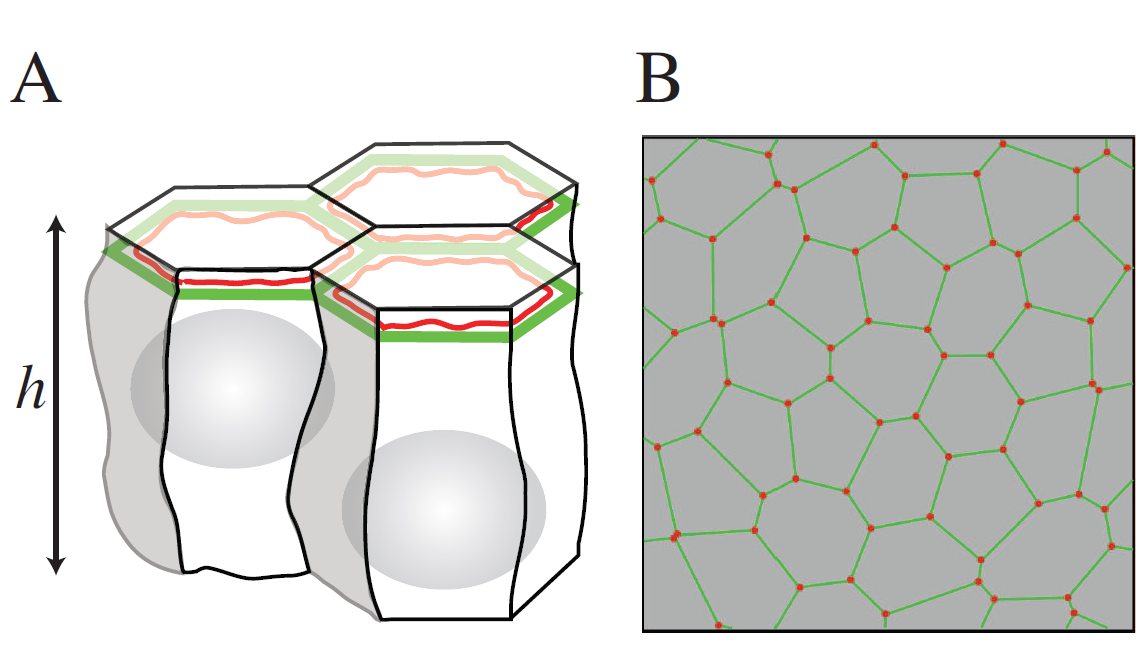
\includegraphics[width=6cm]{twodimensions.png}
    \end{column}
    \begin{column}{\textwidth}
        \begin{enumerate}
        \item < 1-| alert@1 > Epithelia cells are connected to each other via adhesive molecules (\emph{Cadherin}, and components of the \emph{actin cytoskeleton}) near their apical region. 
        \item < 2-| alert@2 > These apical junctions can be considered as a two-dimensional network (\textbf{junctional adherent network}) that defines the cell packing geometry.
        \item < 3-| alert@3 > This 2-dimensional topology makes the study of Epithelia tissues simpler than the study of tissues in 3-dimensions.
        \end{enumerate}
    \end{column}
\end{columns}
\end{minipage}
\end{beamerboxesrounded}
}

\subsection{Real data}
\frame{\frametitle{Tissue growth: cells as polygons, tissues as networks\footnotemark}
\setbeamercolor{uppercol}{fg=black,bg=pink}
\setbeamercolor{lowercol}{fg=black,bg=pink}
\begin{beamerboxesrounded}[upper=upperco,lower=lowercol,shadow=true]{}
\begin{minipage}[t]{6.1cm}
\centering \hspace{4cm}\flashmovie[auto=1,loop=1,controlbar=1,engine=flv-player,width=6cm,height=6cm]{Animation.flv}
\end{minipage}
\end{beamerboxesrounded}
\tiny{\footnotetext[1]{Canine kidney cells (videl kindly offered by Anastasia Trushko (UNIGE))}}
}

\subsection{Theoretical approach}
%%tissue growth remarks
\frame{\frametitle{Tissue, cells, Edges, and Vertices}
\setbeamercolor{uppercol}{fg=black,bg=pink}
\setbeamercolor{lowercol}{fg=black,bg=pink}
\begin{beamerboxesrounded}[upper=upperco,lower=lowercol,shadow=true]{}
\begin{minipage}[t]{6.1cm}
\begin{columns}
    \begin{column}{\textwidth}
        \hspace{0.4cm} 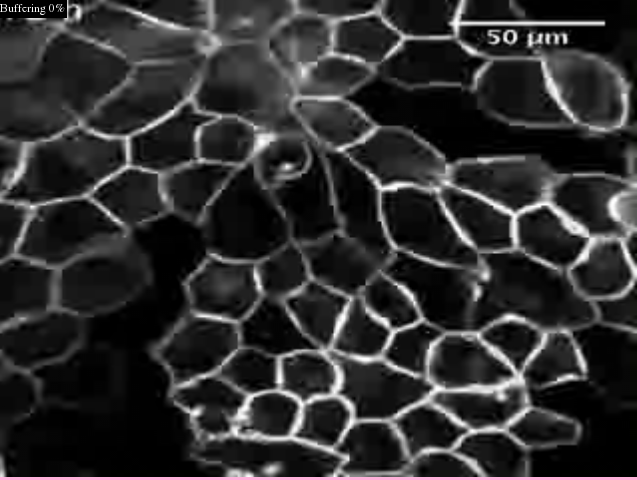
\includegraphics[height=5cm,width=5cm]{network_of_cells.png}
    \end{column}
    \begin{column}{0.8\textwidth}
        \begin{enumerate}
        \item < 1-| alert@1 > Tissue as a network of cells\footnotemark.
        \item < 2-| alert@2 > Cells as polygons\footnotemark[1].
        \item < 3-| alert@1 > Each 2 Cells share 1 Edge\footnotemark[1].
        \item < 4-| alert@2 > Each Edge is composed by 2 Vertices\footnotemark[1].
        \end{enumerate}
    \end{column}
\end{columns}
\end{minipage}
\end{beamerboxesrounded}
\tiny{\footnotetext[1]{Farhadifar et al. \emph{The influence of cell mechanics, cell-cell interactions, and proliferation on epithelial packing.} Current Biology 17.24 (2007): 2095-2104.}}
}

\subsection{Different Kind of tissues}
%%tissue growth remarks
\frame{\frametitle{Cell shapes and Different kind of tissues}
\setbeamercolor{uppercol}{fg=black,bg=pink}
\setbeamercolor{lowercol}{fg=black,bg=pink}
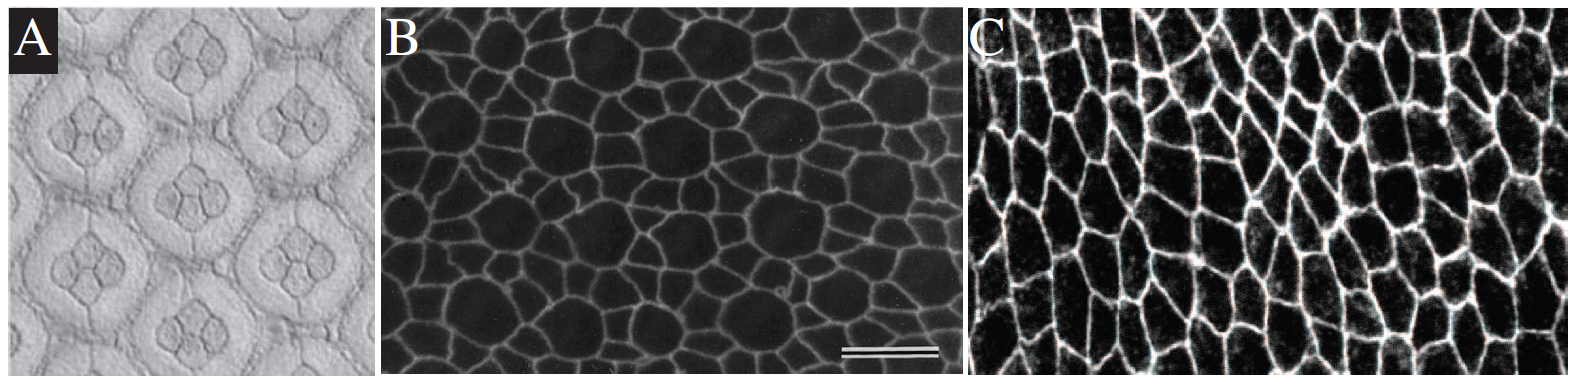
\includegraphics[width=12cm]{./different_tissues.png}\\
\begin{beamerboxesrounded}[upper=upperco,lower=lowercol,shadow=true]{}
\begin{minipage}[t]{8cm}
\begin{columns}
    \begin{column}{\textwidth}
    \begin{enumerate}
       \item A - Drosophila retina ommatidium (eys of a fruit fly)
       \item B - Basilar papilla of chicken embryo
       \item \textbf{C - Drosophila wing disc}
    \end{enumerate}
    \end{column}{\textwidth}
\end{columns}
\end{minipage}
\end{beamerboxesrounded}
}

\subsection{Different Developmental stages}
%%tissue growth remarks
\frame{\frametitle{Cell shapes and Different Developmental stages (Drosophila wings)}
\setbeamercolor{uppercol}{fg=black,bg=pink}
\setbeamercolor{lowercol}{fg=black,bg=pink}
\textbf{(B)} pupal stage \hspace{3.2cm}\textbf{(C)} before hair formation 
\begin{beamerboxesrounded}[upper=upperco,lower=lowercol,shadow=true]{}
\begin{minipage}[t]{6.1cm}
\centering 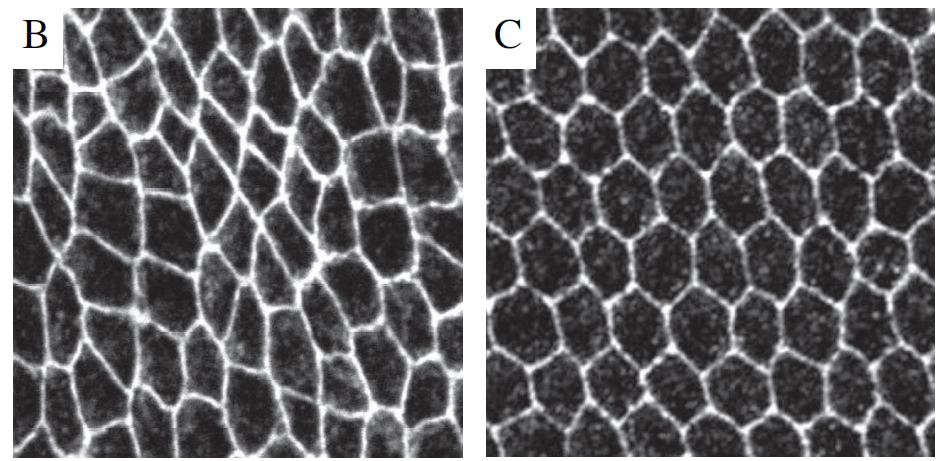
\includegraphics[height=6cm]{./devstages2.png}
\end{minipage}
\end{beamerboxesrounded}
}

\section{General Assumptions}
\subsection{Cell Mechanics}
\frame{\frametitle{Line Tension, Contractility, and Elasticity}
\setbeamercolor{uppercol}{fg=black,bg=pink}
\setbeamercolor{lowercol}{fg=black,bg=pink}
\begin{beamerboxesrounded}[upper=upperco,lower=lowercol,shadow=true]{}
\begin{minipage}[t]{6.5cm}
\begin{columns}
    \begin{column}{\textwidth}
        \hspace{6.5cm}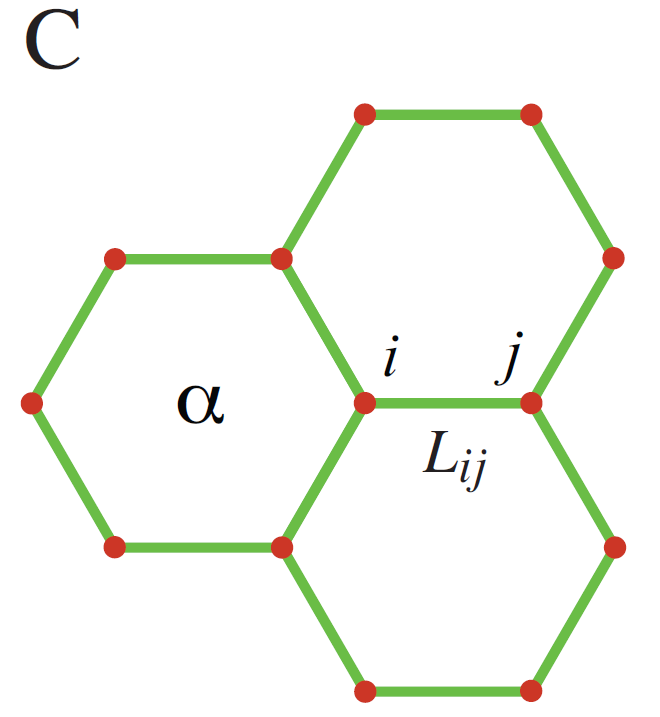
\includegraphics[height=6cm]{./junctionalnetwork_isolated.png}
    \end{column}
    \begin{column}{0.8\textwidth}
        \begin{itemize}
        \item < 1-| alert@1 > Edge's Line tension ($\Lambda$) is associated to Edge's length\footnotemark.
        \item < 2-| alert@2 > Cell's Contractility ($\Gamma$) is associated to Cell's Perimeter\footnotemark[1].
        \item < 3-| alert@3 > Cell's Elasticity ($K$) is associated to Cell's Area\footnotemark[1].
        \end{itemize}
    \end{column}
\end{columns}
\end{minipage}
\end{beamerboxesrounded}
\tiny{\footnotetext[1]{Farhadifar et al. \emph{The influence of cell mechanics, cell-cell interactions, and proliferation on epithelial packing.} Current Biology 17.24 (2007): 2095-2104.}}
}

\subsection{Energy Function}
%%Minimal Energy
\frame{\frametitle{Force Balance Energy Function\footnotemark}
\setbeamercolor{uppercol}{fg=black,bg=pink}
\setbeamercolor{lowercol}{fg=black,bg=pink}
\begin{align*}
\hspace{-0.3cm}F = \tikz[baseline]{\node[fill=blue!20,ellipse,anchor=base] (t1) {$\sum_{\alpha}\frac{K_{\alpha}}{2}(A_{\alpha} - A_{\alpha}^{(0)})^{2}$};} ~ + ~ \tikz[baseline]{\node[fill=yellow!20,ellipse,anchor=base] (t2) {$\sum_{(i,j)}{\Lambda_{ij}L_{ij}}$};}  + \tikz[baseline]{\node[fill=green!20,ellipse,anchor=base] (t3) {$\sum_{\alpha}{\frac{\Gamma_{\alpha}}{2}L_{\alpha}^{2}}$};}
\end{align*}

\begin{itemize}[<+-| alert@+>]
    \item Elasticity and Cell Area ($K_{\alpha}$, and $A_{\alpha}$) 
        \tikz\node[coordinate] (n1) {};
    \item Line tension and Edge length ($\Lambda_{ij}$, and $L_{ij}$)
        \tikz\node[coordinate] (n2) {};
    \item Contractility and Cell Perimeter ($\Gamma_{\alpha}$, and $L_{\alpha}$) 
        \tikz\node[coordinate] (n3) {};
\end{itemize}
% Now it's time to draw some edges between the global nodes. Note that we
% have to apply the 'overlay' style.
%\begin{tikzpicture}[overlay]
%        \path[->]<1-> (n1) edge [bend left] (t1);
%        \path[->]<2-> (n3) edge [out=0, in=-90] (t3);
%        \path[->]<3-> (n2) edge [bend right] (t2);
%\end{tikzpicture}
\tiny{\footnotetext[1]{Farhadifar et al. \emph{The influence of cell mechanics, cell-cell interactions, and proliferation on epithelial packing.} Current Biology 17.24 (2007): 2095-2104.}}
}

%%Minimal Energy

\frame{\frametitle{Force Balance Energy Function\footnotemark}
\setbeamercolor{uppercol}{fg=black,bg=pink}
\setbeamercolor{lowercol}{fg=black,bg=pink}
\begin{align*}
\hspace{-0.3cm}F = \tikz[baseline]{\node[fill=blue!20,ellipse,anchor=base] (t1) {$\sum_{\alpha}\frac{K_{\alpha}}{2}(A_{\alpha} - A_{\alpha}^{(0)})^{2}$};} ~ + ~ \tikz[baseline]{\node[fill=yellow!20,ellipse,anchor=base] (t2) {$\sum_{(i,j)}{\Lambda_{ij}L_{ij}}$};}  + \tikz[baseline]{\node[fill=green!20,ellipse,anchor=base] (t3) {$\sum_{\alpha}{\frac{\Gamma_{\alpha}}{2}L_{\alpha}^{2}}$};}
\end{align*}
%$F = \sum_{\alpha}{\frac{K_{\alpha}}{2}(A_{\alpha} - A_{\alpha}^{(0)})^{2} ~ + ~ \sum_{(i,j)}{\Lambda_{ij}L_{ij}} ~ + ~  \sum_{\alpha}{\frac{\Gamma_{\alpha}}{2}L_{\alpha}^{2}}}$
\begin{beamerboxesrounded}[upper=upperco,lower=lowercol,shadow=true]{}
\begin{minipage}[t]{6.1cm}
\begin{columns}
    \begin{column}{\textwidth}
       \hspace{0.4cm} 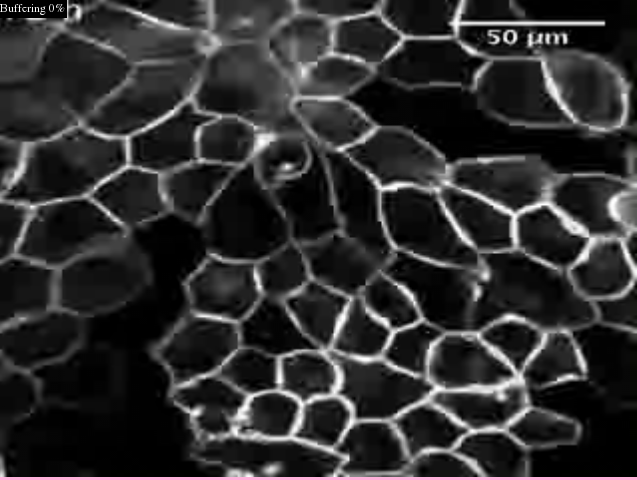
\includegraphics[height=5cm,width=5cm]{network_of_cells.png}
    \end{column}
    \begin{column}{0.8\textwidth}
       The physical properties of the cells are static. So, in order to satisfy the \textbf{Minimal Energy's Assumption} the positions of the vertices change for different combination of parameters and different events (like the appearance of new cells).
    \end{column}
\end{columns}
\end{minipage}
\end{beamerboxesrounded}
\tiny{\footnotetext[1]{Farhadifar et al. \emph{The influence of cell mechanics, cell-cell interactions, and proliferation on epithelial packing.} Current Biology 17.24 (2007): 2095-2104.}}
}

%%Minimal Energy
\frame{\frametitle{Preferred Cell's Area $A_{\alpha}^{(0)}$\footnotemark}
\setbeamercolor{uppercol}{fg=black,bg=pink}
\setbeamercolor{lowercol}{fg=black,bg=pink}
%$F = \sum_{\alpha}{\frac{K_{\alpha}}{2}(A_{\alpha} - A_{\alpha}^{(0)})^{2} ~ + ~ \sum_{(i,j)}{\Lambda_{ij}L_{ij}} ~ + ~  \sum_{\alpha}{\frac{\Gamma_{\alpha}}{2}L_{\alpha}^{2}}}$
\begin{align*}
\hspace{-0.3cm}F = \tikz[baseline]{\node[fill=blue!20,ellipse,anchor=base] (t1) {$\sum_{\alpha}\frac{K_{\alpha}}{2}(A_{\alpha} - A_{\alpha}^{(0)})^{2}$};} ~ + ~ \tikz[baseline]{\node[fill=yellow!20,ellipse,anchor=base] (t2) {$\sum_{(i,j)}{\Lambda_{ij}L_{ij}}$};}  + \tikz[baseline]{\node[fill=green!20,ellipse,anchor=base] (t3) {$\sum_{\alpha}{\frac{\Gamma_{\alpha}}{2}L_{\alpha}^{2}}$};}
\end{align*}
\begin{beamerboxesrounded}[upper=upperco,lower=lowercol,shadow=true]{}
\begin{minipage}[t]{6.1cm}
\begin{columns}
    \begin{column}{\textwidth}
       \hspace{0.4cm} 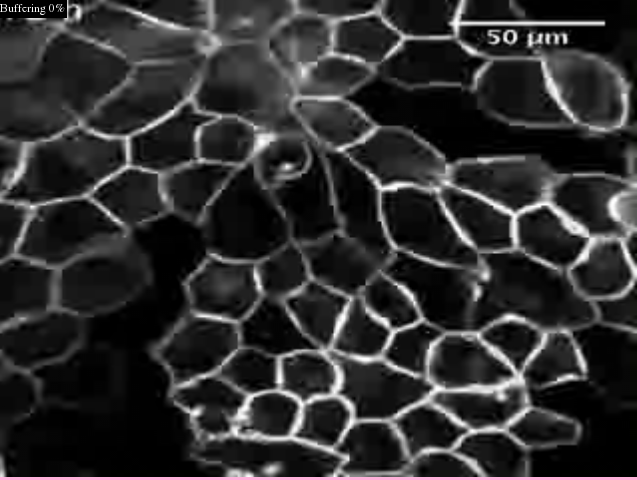
\includegraphics[height=5cm,width=5cm]{network_of_cells.png}
    \end{column}
    \begin{column}{0.8\textwidth}
    $A_{\alpha}^{(0)}$ is the preferred area of cell $\alpha$ which is related to the volume, $V_{\alpha}$ and height, $h_{\alpha}$ of the cell: $A_{\alpha}^{(0)} ~ = ~ \frac{V_{\alpha}}{h_{\alpha}} $
    \end{column}
\end{columns}
\end{minipage}
\end{beamerboxesrounded}
\tiny{\footnotetext[1]{Farhadifar et al. \emph{The influence of cell mechanics, cell-cell interactions, and proliferation on epithelial packing.} Current Biology 17.24 (2007): 2095-2104.}}
}

\section{Question}
%%tissue growth remarks
\frame{\frametitle{Robustness question}
\setbeamercolor{uppercol}{fg=black,bg=pink}
\setbeamercolor{lowercol}{fg=black,bg=pink}
\begin{beamerboxesrounded}[upper=upperco,lower=lowercol,shadow=true]{}
\begin{minipage}[t]{10cm}
How do mechanical properties of cells (Cells elasticity, Cells contractility, Edges line tension) affect the growth of tissues? 
\end{minipage}
\end{beamerboxesrounded}
}

\frame{\frametitle{Strategy to answer the question}
\setbeamercolor{uppercol}{fg=black,bg=pink}
\setbeamercolor{lowercol}{fg=black,bg=pink}
To explore a broad range of mechanical parameters (at high resolution) and study the effects of such parameters in the characteristics (\textbf{Phenotype}) of simulated cells and tissues.
\begin{beamerboxesrounded}[upper=upperco,lower=lowercol,shadow=true]{}
\begin{minipage}[t]{10cm}
\textbf{Potential phenotypes to study:}
\begin{itemize}
\item < 1-| alert@1 > Cells shape distribution.
\item < 2-| alert@2 > Cells area distribution.
\item < 3-| alert@3 > Cells perimeter distribution.
\item < 4-| alert@4 > Cells \emph{regularity} distribution.
\item < 5-| alert@5 > Edges angle distribution.
\end{itemize}
\end{minipage}
\end{beamerboxesrounded}
}

\section{Model Dynamics}
\subsection{Sequence of Events}
%%tissue growth remarks
\frame{\frametitle{Sequence of Events\footnotemark}
\setbeamercolor{uppercol}{fg=black,bg=pink}
\setbeamercolor{lowercol}{fg=black,bg=pink}
\begin{beamerboxesrounded}[upper=upperco,lower=lowercol,shadow=true]{}
\begin{minipage}[t]{8cm}
\begin{columns}
    \begin{column}{\textwidth}
        \small{\textbf{1 - Relaxation}\\ Vertices change their position to guarantee the force balance to be equal to zero.}
        \hspace{4cm}\flashmovie[auto=1,loop=1,controlbar=1,engine=flv-player,width=5cm,height=5cm]{regular_relaxation.flv}
    \end{column}
    \begin{column}{0.8\textwidth}
        \small{\textbf{2 - Cell Proliferation}\\ cells growth and cells division.\\}
        \flashmovie[auto=1,loop=1,controlbar=1,engine=flv-player,width=5cm,height=5cm]{celldivision.flv}
    \end{column}
\end{columns}
\end{minipage}
\end{beamerboxesrounded}
\tiny{\footnotetext[1]{Farhadifar et al. \emph{The influence of cell mechanics, cell-cell interactions, and proliferation on epithelial packing.} Current Biology 17.24 (2007): 2095-2104.}}
}


\frame{\frametitle{Initial conditions and constrains}
\setbeamercolor{uppercol}{fg=black,bg=pink}
\setbeamercolor{lowercol}{fg=black,bg=pink}
\begin{beamerboxesrounded}[upper=upperco,lower=lowercol,shadow=true]{}
\begin{minipage}[t]{10cm}
\begin{enumerate}
\item < 1-| alert@1 > Rectangular tissue with regular hexagonal cells (all the edges of the cells have the same length).
\item < 2-| alert@2 > Non-boundary periodic conditions (the tissue is not \emph{infinite}).
\item < 3-| alert@3 > Line tension of boundary cells ($\Lambda_{b}$) is half the value of the other cells\footnotemark.
\end{enumerate}
\end{minipage}
\end{beamerboxesrounded}
%\tiny{\footnotetext[1]{Farhadifar et al. \emph{The influence of cell mechanics, cell-cell interactions, and proliferation on epithelial packing.} Current Biology 17.24 (2007): 2095-2104.}}
}


\section{Relaxation}
\subsection{Relaxation}
%%tissue growth remarks
\frame{\frametitle{Relaxation\footnotemark}
\setbeamercolor{uppercol}{fg=black,bg=pink}
\setbeamercolor{lowercol}{fg=black,bg=pink}
\begin{beamerboxesrounded}[upper=upperco,lower=lowercol,shadow=true]{}
\begin{minipage}[t]{6.1cm}
\begin{columns}
    \begin{column}{\textwidth}
        \hspace{1cm}\flashmovie[auto=1,loop=1,controlbar=1,engine=flv-player,width=6cm,height=6cm]{regular_relaxation.flv}
    \end{column}
    \begin{column}{0.8\textwidth}
        \begin{itemize}
        \item 1 - Vertices change their position to guarantee the force balance equal to zero.
        \end{itemize}
    \end{column}
\end{columns}
\end{minipage}
\end{beamerboxesrounded}
\tiny{\footnotetext[1]{Farhadifar et al. \emph{The influence of cell mechanics, cell-cell interactions, and proliferation on epithelial packing.} Current Biology 17.24 (2007): 2095-2104.}}
}


%%tissue growth remarks
\frame{\frametitle{Relaxation\footnotemark}
\setbeamercolor{uppercol}{fg=black,bg=pink}
\setbeamercolor{lowercol}{fg=black,bg=pink}
\begin{beamerboxesrounded}[upper=upperco,lower=lowercol,shadow=true]{}
\begin{minipage}[t]{6.1cm}
\begin{columns}
    \begin{column}{\textwidth}
        \hspace{1cm}\flashmovie[auto=1,loop=1,controlbar=1,engine=flv-player,width=6cm,height=6cm]{regular_relaxation.flv}
    \end{column}
    \begin{column}{0.8\textwidth}
        \begin{itemize}
        \item 2 - The position of the vertices is defined by a \emph{Verlet Function} in which the accelleration is defined by the total force on the junctions of the tissue.
        \end{itemize}
    \end{column}
\end{columns}
\end{minipage}
\end{beamerboxesrounded}
\tiny{\footnotetext[1]{Farhadifar et al. \emph{The influence of cell mechanics, cell-cell interactions, and proliferation on epithelial packing.} Current Biology 17.24 (2007): 2095-2104.}}
}


%%tissue growth remarks
\frame{\frametitle{Relaxation\footnotemark}
\setbeamercolor{uppercol}{fg=black,bg=pink}
\setbeamercolor{lowercol}{fg=black,bg=pink}
\begin{beamerboxesrounded}[upper=upperco,lower=lowercol,shadow=true]{}
\begin{minipage}[t]{6.1cm}
\begin{columns}
    \begin{column}{\textwidth}
        \hspace{1cm}\flashmovie[auto=1,loop=1,controlbar=1,engine=flv-player,width=6cm,height=6cm]{regular_relaxation.flv}
    \end{column}
    \begin{column}{0.8\textwidth}
        \begin{itemize}
        \item 3 - Once the force is zero, the accelleration of the \emph{Verlet Function} is also zero, and so the position of the vertices don't change from time step $t$ to $t + \Delta t$. 
        \end{itemize}
    \end{column}
\end{columns}
\end{minipage}
\end{beamerboxesrounded}
\tiny{\footnotetext[1]{Farhadifar et al. \emph{The influence of cell mechanics, cell-cell interactions, and proliferation on epithelial packing.} Current Biology 17.24 (2007): 2095-2104.}}
}

%%tissue growth remarks
\frame{\frametitle{Relaxation}
\setbeamercolor{uppercol}{fg=black,bg=pink}
\setbeamercolor{lowercol}{fg=black,bg=pink}
\begin{beamerboxesrounded}[upper=upperco,lower=lowercol,shadow=true]{}
\begin{minipage}[t]{6.1cm}
\begin{columns}
    \begin{column}{\textwidth}
        \hspace{1cm}\flashmovie[auto=1,loop=1,controlbar=1,engine=flv-player,width=6cm,height=6cm]{regular_relaxation.flv}
    \end{column}
    \begin{column}{0.8\textwidth}
        \begin{itemize}
        \item 4 - Relaxation is finished once the length of the tissue remains \emph{steady} (the position of its vertices don't change) along 100 time steps ($\frac{sd(\sum_{\alpha}{L_{\alpha}})}{mean({\sum_{\alpha}{L_{\alpha}}})} \apeq 0 $).
        \end{itemize}
    \end{column}
\end{columns}
\end{minipage}
\end{beamerboxesrounded}
}


%%tissue growth remarks
\frame{\frametitle{\emph{Regularness of the tissue}}
\setbeamercolor{uppercol}{fg=black,bg=pink}
\setbeamercolor{lowercol}{fg=black,bg=pink}
\begin{beamerboxesrounded}[upper=upperco,lower=lowercol,shadow=true]{}
\begin{minipage}[t]{10cm}
    \begin{enumerate}
    \item < 1-| alert@1 > We define \textbf{\emph{regularity}} as a dimensionless measure to say how regular the cells of a tissue are.
    \item < 2-| alert@1 > Regularness is defined as: $Reg = \frac{sd(L_{ij})}{mean(L_{ij})}$ accross all the edges.
    \end{enumerate}
\end{minipage}
\end{beamerboxesrounded}
}


%%tissue growth remarks
\frame{\frametitle{\emph{Regularness of the tissue}}
\setbeamercolor{uppercol}{fg=black,bg=pink}
\setbeamercolor{lowercol}{fg=black,bg=pink}
We define \textbf{\emph{regularity}} as a dimensionless measure to say how regular the cells of a tissue are.
\begin{beamerboxesrounded}[upper=upperco,lower=lowercol,shadow=true]{}
\begin{minipage}[t]{8cm}
\begin{columns}
    \begin{column}{\textwidth}
        \small{$Reg ~ \apeq ~ 0$\\
        $(Lambda,Gamma) = (0,0.15)$}
        \flashmovie[auto=1,loop=1,controlbar=1,engine=flv-player,width=5cm,height=5cm]{regular_relaxation.flv}
    \end{column}
    \begin{column}{0.8\textwidth}
        \small{$Reg ~ > ~ 0$\\
        $(-0.6,0.08)$}
        \flashmovie[auto=1,loop=1,controlbar=1,engine=flv-player,width=5cm,height=5cm]{soft_relaxation.flv}
    \end{column}
\end{columns}
\end{minipage}
\end{beamerboxesrounded}
}


%%tissue growth remarks
\frame{\frametitle{\emph{Phase space of Regularness}}
\setbeamercolor{uppercol}{fg=black,bg=pink}
\setbeamercolor{lowercol}{fg=black,bg=pink}
\begin{beamerboxesrounded}[upper=upperco,lower=lowercol,shadow=true]{}
\centering \hspace{4cm} 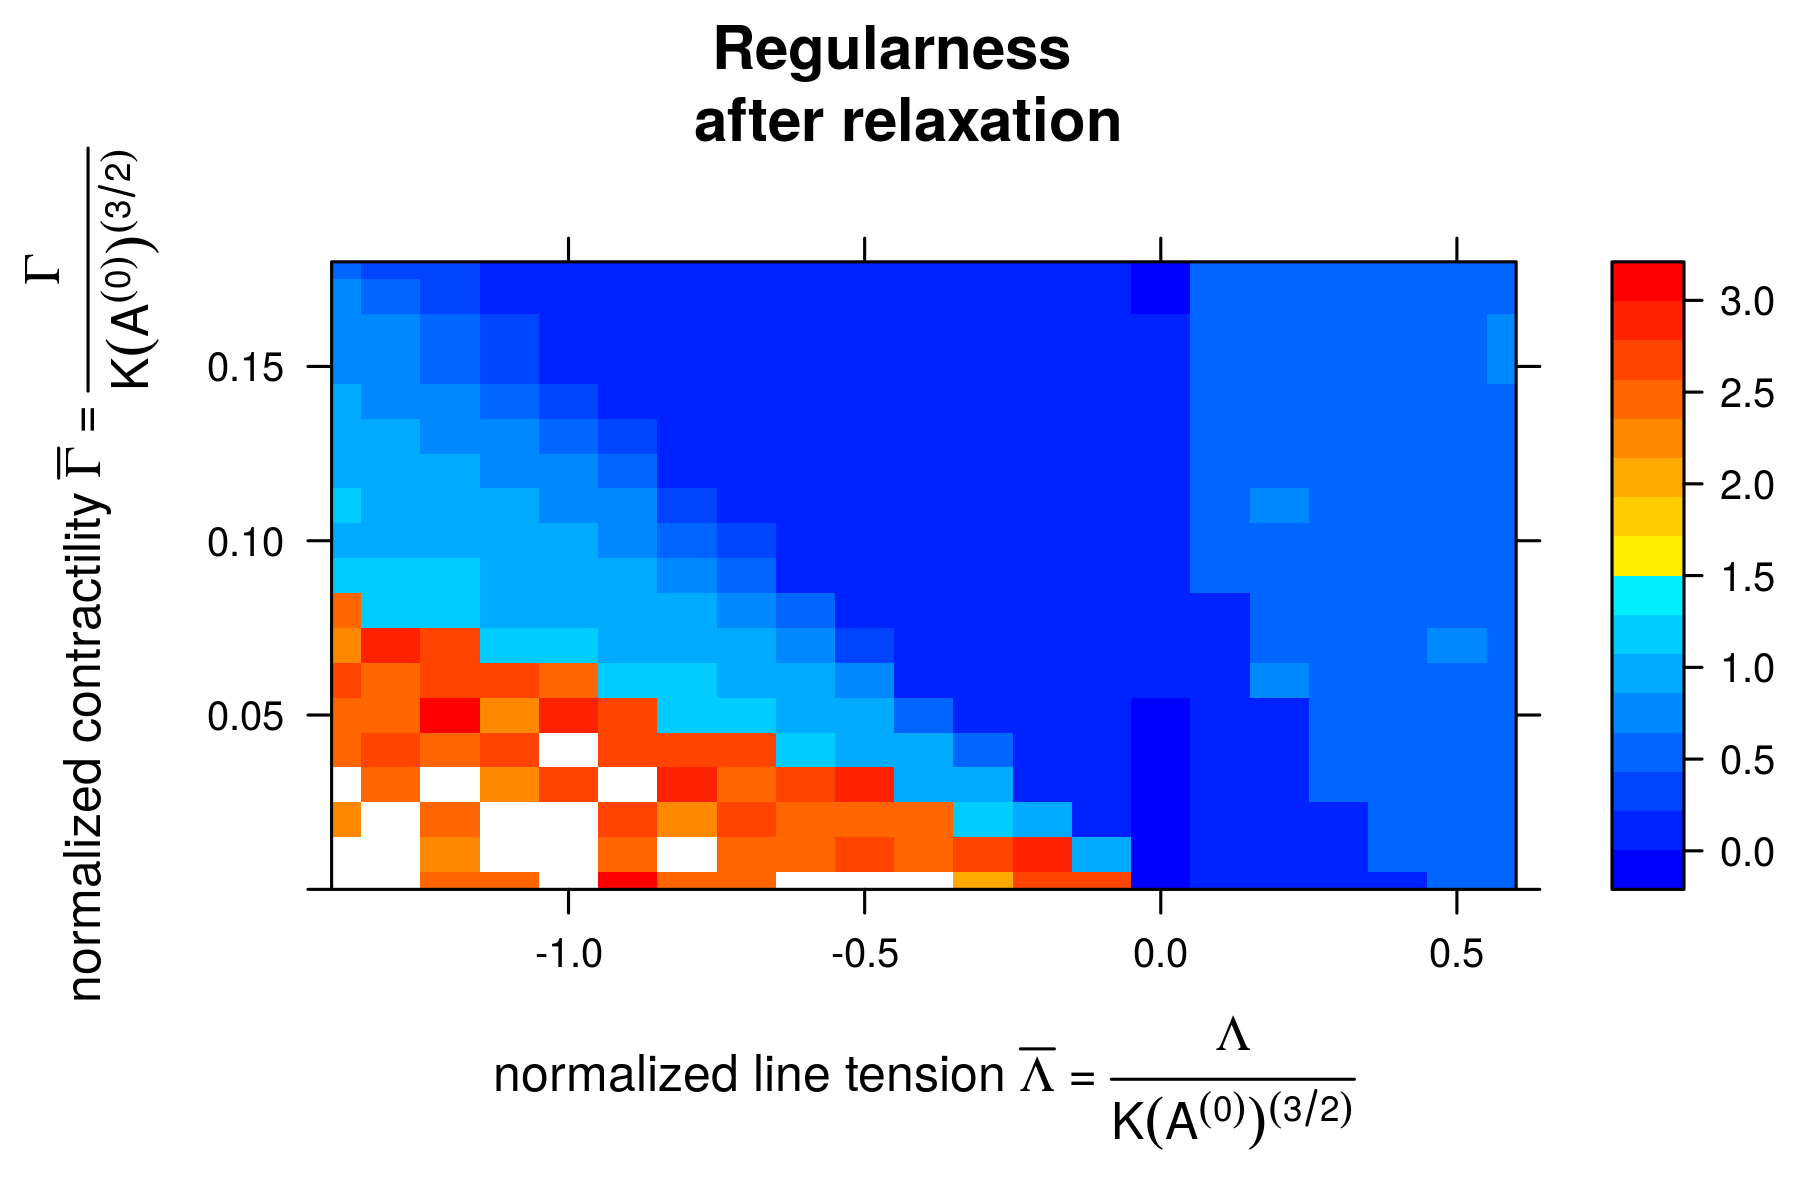
\includegraphics[width=10cm]{levelplot_reg_relaxation.png}
\end{beamerboxesrounded}
}


%%%tissue growth remarks
%\frame{\frametitle{\emph{Phase space of Regularness in Time}}
%\setbeamercolor{uppercol}{fg=black,bg=pink}
%\setbeamercolor{lowercol}{fg=black,bg=pink}
%\begin{beamerboxesrounded}[upper=upperco,lower=lowercol,shadow=true]{}
%\begin{minipage}[t]{6.1cm}
%\centering \flashmovie[auto=0,loop=1,controlbar=1,engine=flv-player,width=6cm,height=6cm]{Animation.flv}
%\end{minipage}
%\end{beamerboxesrounded}
%}



%%%%%%%% CELL DIVISION

\section{Cell Proliferation}
\subsection{Cell Proliferation}
%%tissue growth remarks
\frame{\frametitle{Cell Proliferation}
\setbeamercolor{uppercol}{fg=black,bg=pink}
\setbeamercolor{lowercol}{fg=black,bg=pink}
\begin{beamerboxesrounded}[upper=upperco,lower=lowercol,shadow=true]{}
\begin{minipage}[t]{6.1cm}
\begin{columns}
    \begin{column}{\textwidth}
        \hspace{1cm}\flashmovie[auto=1,loop=1,controlbar=1,engine=flv-player,width=6cm,height=6cm]{celldivision.flv}
    \end{column}
    \begin{column}{0.8\textwidth}
        \begin{itemize}
        \item Cell Growth.
        \item Cell Division.
        \end{itemize}
    \end{column}
\end{columns}
\end{minipage}
\end{beamerboxesrounded}
}


\subsection{Cell Growth}
%%tissue growth remarks
\frame{\frametitle{Cell Growth\footnotemark}
\setbeamercolor{uppercol}{fg=black,bg=pink}
\setbeamercolor{lowercol}{fg=black,bg=pink}
\begin{beamerboxesrounded}[upper=upperco,lower=lowercol,shadow=true]{}
\begin{minipage}[t]{6.1cm}
\begin{columns}
    \begin{column}{\textwidth}
        \hspace{4cm} 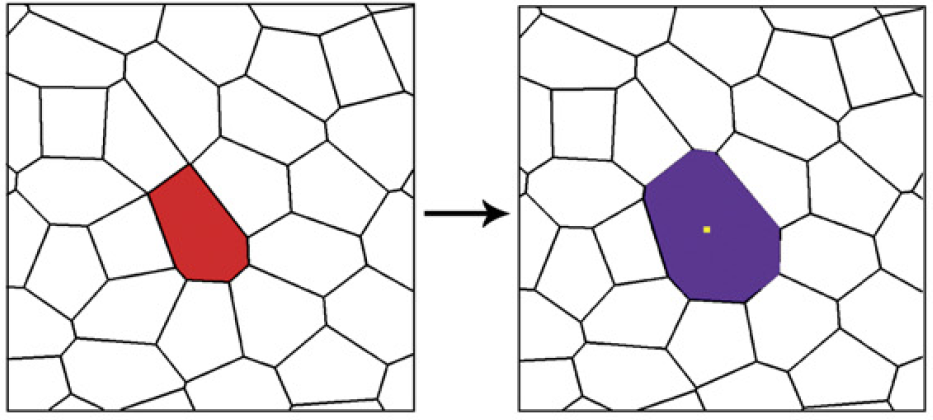
\includegraphics[width=6cm]{cellgrowth.png}
    \end{column}
    \begin{column}{0.8\textwidth}
        \begin{enumerate}
        \item < 1-| alert@1 > Cells are \textbf{randomly} triggered to increase their area.
        \item < 2-| alert@2 > They increase their area by 10\% each time step.
        \end{enumerate}
    \end{column}
\end{columns}
\end{minipage}
\end{beamerboxesrounded}
\tiny{\footnotetext[1]{Farhadifar et al. \emph{The influence of cell mechanics, cell-cell interactions, and proliferation on epithelial packing.} Current Biology 17.24 (2007): 2095-2104.}}
}

%%tissue growth remarks
\frame{\frametitle{Cell Growth\footnotemark}
\setbeamercolor{uppercol}{fg=black,bg=pink}
\setbeamercolor{lowercol}{fg=black,bg=pink}
\begin{beamerboxesrounded}[upper=upperco,lower=lowercol,shadow=true]{}
\begin{minipage}[t]{6.1cm}
\begin{columns}
    \begin{column}{\textwidth}
        \hspace{4cm} 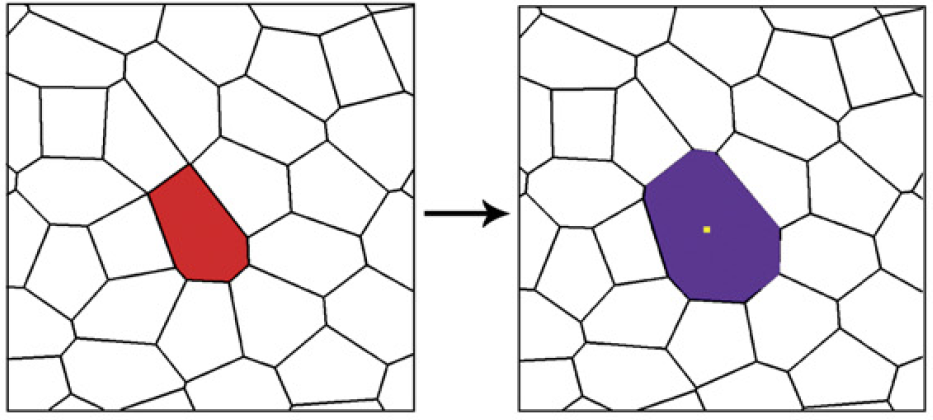
\includegraphics[width=6cm]{cellgrowth.png}
    \end{column}
    \begin{column}{0.8\textwidth}
        \begin{enumerate}
        \item < 1-| alert@1 > The increment of the area is given by changing the value of the preferred area parameter ($A_{\alpha}^{(0)}$) on the Force balance equation.
        \end{enumerate}
    \end{column}
\end{columns}
\end{minipage}
\end{beamerboxesrounded}
\tiny{\footnotetext[1]{Farhadifar et al. \emph{The influence of cell mechanics, cell-cell interactions, and proliferation on epithelial packing.} Current Biology 17.24 (2007): 2095-2104.}}
}

\subsection{Cell Division}
%%tissue growth remarks
\frame{\frametitle{Cell Division\footnotemark}
\setbeamercolor{uppercol}{fg=black,bg=pink}
\setbeamercolor{lowercol}{fg=black,bg=pink}
\begin{beamerboxesrounded}[upper=upperco,lower=lowercol,shadow=true]{}
\begin{minipage}[t]{6.1cm}
\begin{columns}
    \begin{column}{\textwidth}
        \hspace{4cm} 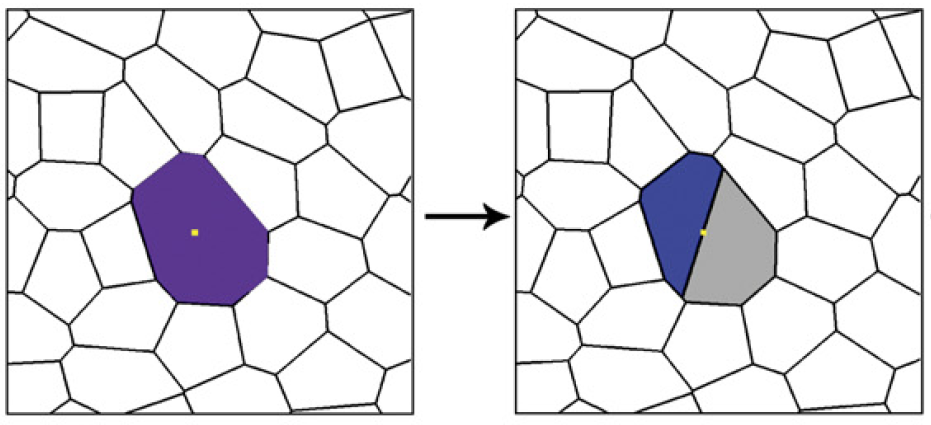
\includegraphics[width=6cm]{celldivision.png}
    \end{column}
    \begin{column}{0.8\textwidth}
        \begin{enumerate}
        \item < 1-| alert@1 > Once a cell $\alpha$ reaches the \textbf{double} of the area it had \textbf{before starting to increase}, it is subdivided into two cells with half the current area of cell $\alpha$.
        \end{enumerate}
    \end{column}
\end{columns}
\end{minipage}
\end{beamerboxesrounded}
\tiny{\footnotetext[1]{Farhadifar et al. \emph{The influence of cell mechanics, cell-cell interactions, and proliferation on epithelial packing.} Current Biology 17.24 (2007): 2095-2104.}}
}

%%tissue growth remarks
\frame{\frametitle{Cell Division\footnotemark}
\setbeamercolor{uppercol}{fg=black,bg=pink}
\setbeamercolor{lowercol}{fg=black,bg=pink}
\begin{beamerboxesrounded}[upper=upperco,lower=lowercol,shadow=true]{}
\begin{minipage}[t]{6.1cm}
\begin{columns}
    \begin{column}{\textwidth}
        \hspace{4cm} 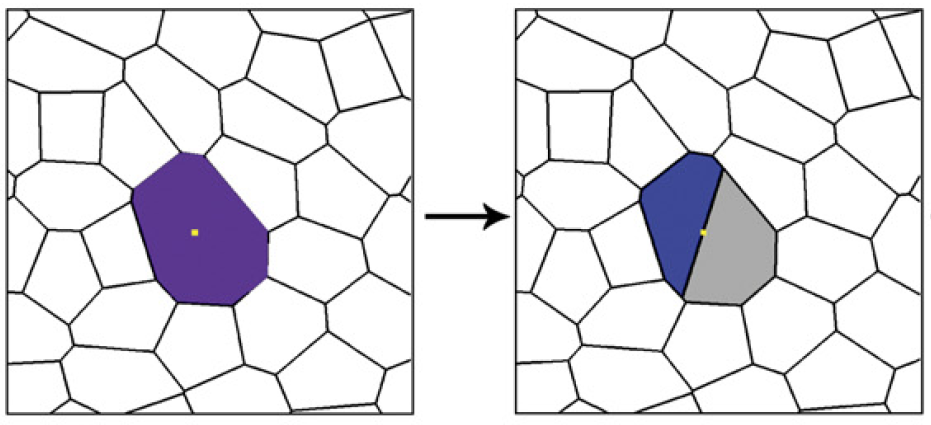
\includegraphics[width=6cm]{celldivision.png}
    \end{column}
    \begin{column}{0.8\textwidth}
        \begin{enumerate}
        \item < 1-| alert@1 > The division consists in creating a new edge $e_{i}$ that \textbf{crosses the centroid} of the original cell $\alpha$ with a \textbf{random direction}.
        \end{enumerate}
    \end{column}
\end{columns}
\end{minipage}
\end{beamerboxesrounded}
\tiny{\footnotetext[1]{Farhadifar et al. \emph{The influence of cell mechanics, cell-cell interactions, and proliferation on epithelial packing.} Current Biology 17.24 (2007): 2095-2104.}}
}


%%tissue growth remarks
\frame{\frametitle{Cell Division\footnotemark}
\setbeamercolor{uppercol}{fg=black,bg=pink}
\setbeamercolor{lowercol}{fg=black,bg=pink}
\begin{beamerboxesrounded}[upper=upperco,lower=lowercol,shadow=true]{}
\begin{minipage}[t]{6.1cm}
\begin{columns}
    \begin{column}{\textwidth}
        \hspace{4cm} 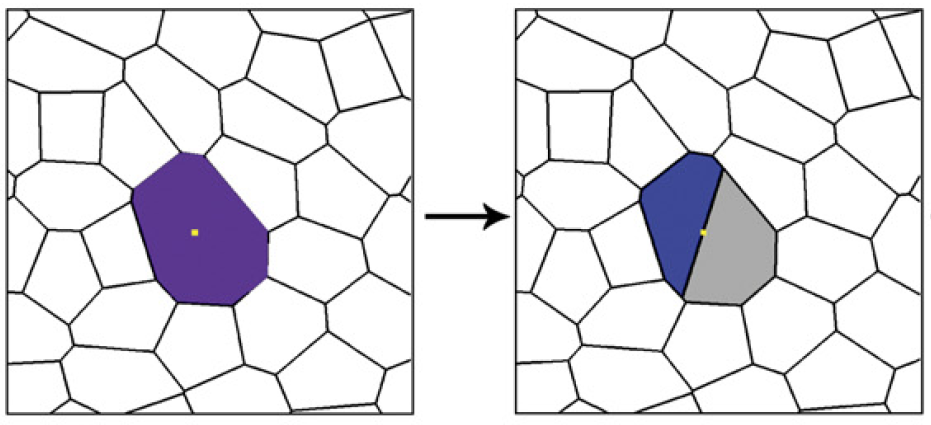
\includegraphics[width=6cm]{celldivision.png}
    \end{column}
    \begin{column}{0.8\textwidth}
        \begin{enumerate}
        \item < 1-| alert@1 > The former cell $\alpha$ is replaced by two new cells that share the edge $e_{i}$.
        \end{enumerate}
    \end{column}
\end{columns}
\end{minipage}
\end{beamerboxesrounded}
\tiny{\footnotetext[1]{Farhadifar et al. \emph{The influence of cell mechanics, cell-cell interactions, and proliferation on epithelial packing.} Current Biology 17.24 (2007): 2095-2104.}}
}


%%tissue growth remarks
\frame{\frametitle{Cell Division\footnotemark}
\setbeamercolor{uppercol}{fg=black,bg=pink}
\setbeamercolor{lowercol}{fg=black,bg=pink}
\begin{beamerboxesrounded}[upper=upperco,lower=lowercol,shadow=true]{}
\begin{minipage}[t]{6.1cm}
\begin{columns}
    \begin{column}{\textwidth}
        \hspace{4cm} 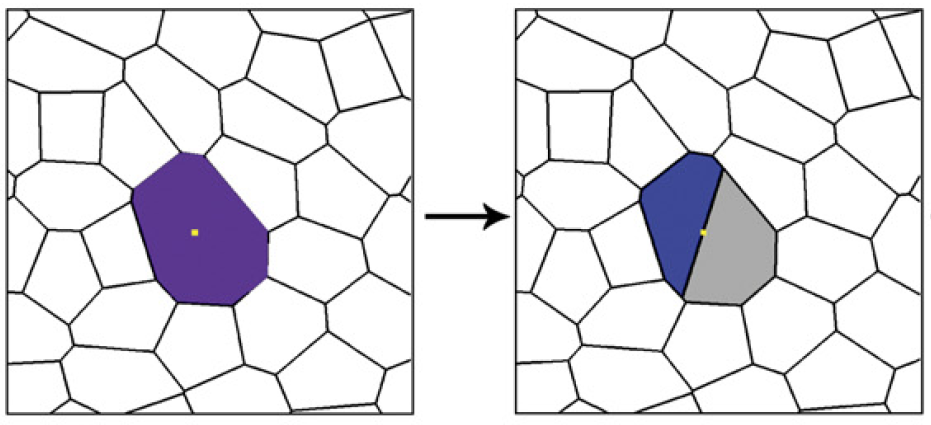
\includegraphics[width=6cm]{celldivision.png}
    \end{column}
    \begin{column}{0.8\textwidth}
        \begin{enumerate}
        \item < 1-| alert@1 > Edges in neighbour cells that are now connected to one of the vertices of $e_{i}$ need to be splitted into two edges.
        \end{enumerate}
    \end{column}
\end{columns}
\end{minipage}
\end{beamerboxesrounded}
\tiny{\footnotetext[1]{Farhadifar et al. \emph{The influence of cell mechanics, cell-cell interactions, and proliferation on epithelial packing.} Current Biology 17.24 (2007): 2095-2104.}}
}


%%tissue growth remarks
\frame{\frametitle{Cell Division\footnotemark}
\setbeamercolor{uppercol}{fg=black,bg=pink}
\setbeamercolor{lowercol}{fg=black,bg=pink}
\begin{beamerboxesrounded}[upper=upperco,lower=lowercol,shadow=true]{}
\begin{minipage}[t]{6.1cm}
\begin{columns}
    \begin{column}{\textwidth}
        \hspace{4cm} 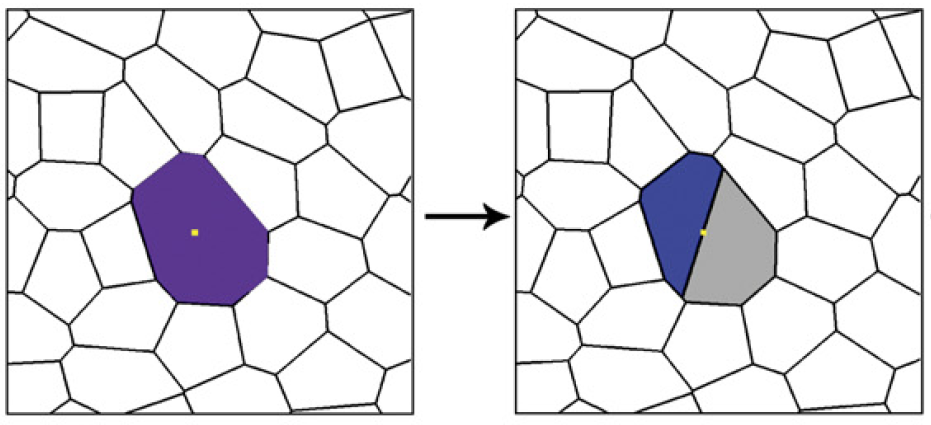
\includegraphics[width=6cm]{celldivision.png}
    \end{column}
    \begin{column}{0.8\textwidth}
        \begin{enumerate}
        \item < 1-| alert@1 > This procedure changes the \emph{shape} of the cells in the neighbourhood of $\alpha$, as well as it creates new cells to replace $\alpha$ that not necessarily have the same \emph{shape} as $\alpha$.
        \end{enumerate}
    \end{column}
\end{columns}
\end{minipage}
\end{beamerboxesrounded}
\tiny{\footnotetext[1]{Farhadifar et al. \emph{The influence of cell mechanics, cell-cell interactions, and proliferation on epithelial packing.} Current Biology 17.24 (2007): 2095-2104.}}
}


\subsection{Steady State}
%%tissue growth remarks
\frame{\frametitle{Steady state}
\setbeamercolor{uppercol}{fg=black,bg=pink}
\setbeamercolor{lowercol}{fg=black,bg=pink}
\begin{beamerboxesrounded}[upper=upperco,lower=lowercol,shadow=true]{}
\begin{minipage}[t]{6.1cm}
\begin{columns}
    \begin{column}{\textwidth}
        \hspace{4cm} 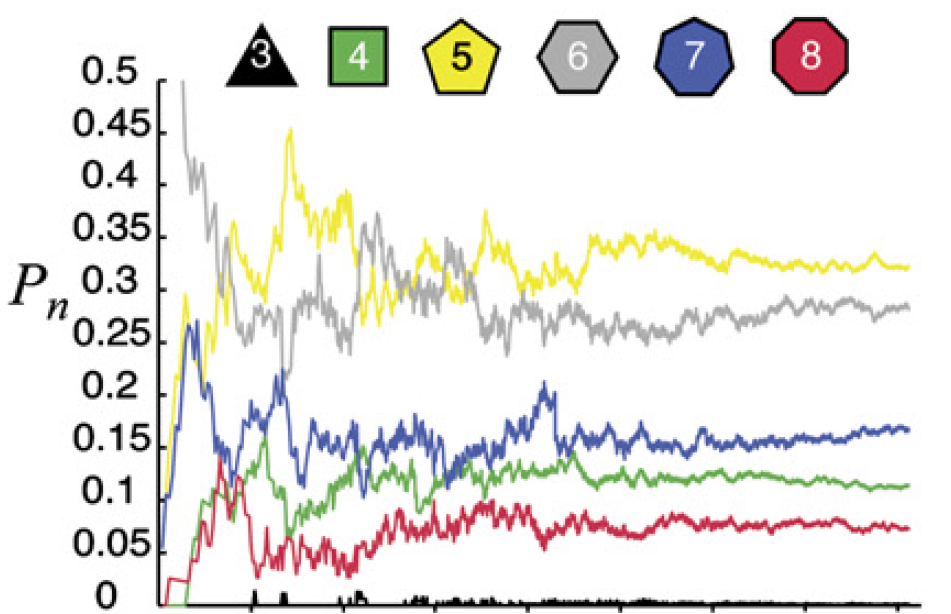
\includegraphics[width=6cm]{timeseries.png}
    \end{column}
    \begin{column}{0.8\textwidth}
        \begin{enumerate}
        \item < 1-| alert@1 > The steady state of the cell division proccess is observed once the relative proportion of cells don't change along 100 time steps.
        \end{enumerate}
    \end{column}
\end{columns}
\end{minipage}
\end{beamerboxesrounded}
}

\subsection{Results}
%%tissue growth remarks
\frame{\frametitle{Change in shapes distribution}
\setbeamercolor{uppercol}{fg=black,bg=pink}
\setbeamercolor{lowercol}{fg=black,bg=pink}
\begin{minipage}[t]{8cm}
\begin{columns}
    \begin{column}{\textwidth}
        \small{$Reg ~ \apeq ~ 0$\\
        $(Lambda,Gamma) = (0,0.15)$}
        \flashmovie[auto=1,loop=1,controlbar=1,engine=flv-player,width=5cm,height=5cm]{shapedistribution1.flv}
    \end{column}
    \begin{column}{\textwidth}
        \small{$Reg ~ > ~ 0$\\
        $(-0.6,0.08)$}
        \flashmovie[auto=1,loop=1,controlbar=1,engine=flv-player,width=5cm,height=5cm]{shapedistribution2.flv}
    \end{column}
\end{columns}
\end{minipage}
}


%%tissue growth remarks
\frame{\frametitle{Phase space: Mean shape of cells (5 Repl.)}
\setbeamercolor{uppercol}{fg=black,bg=pink}
\setbeamercolor{lowercol}{fg=black,bg=pink}
\begin{beamerboxesrounded}[upper=upperco,lower=lowercol,shadow=true]{}
\centering \hspace{4cm} 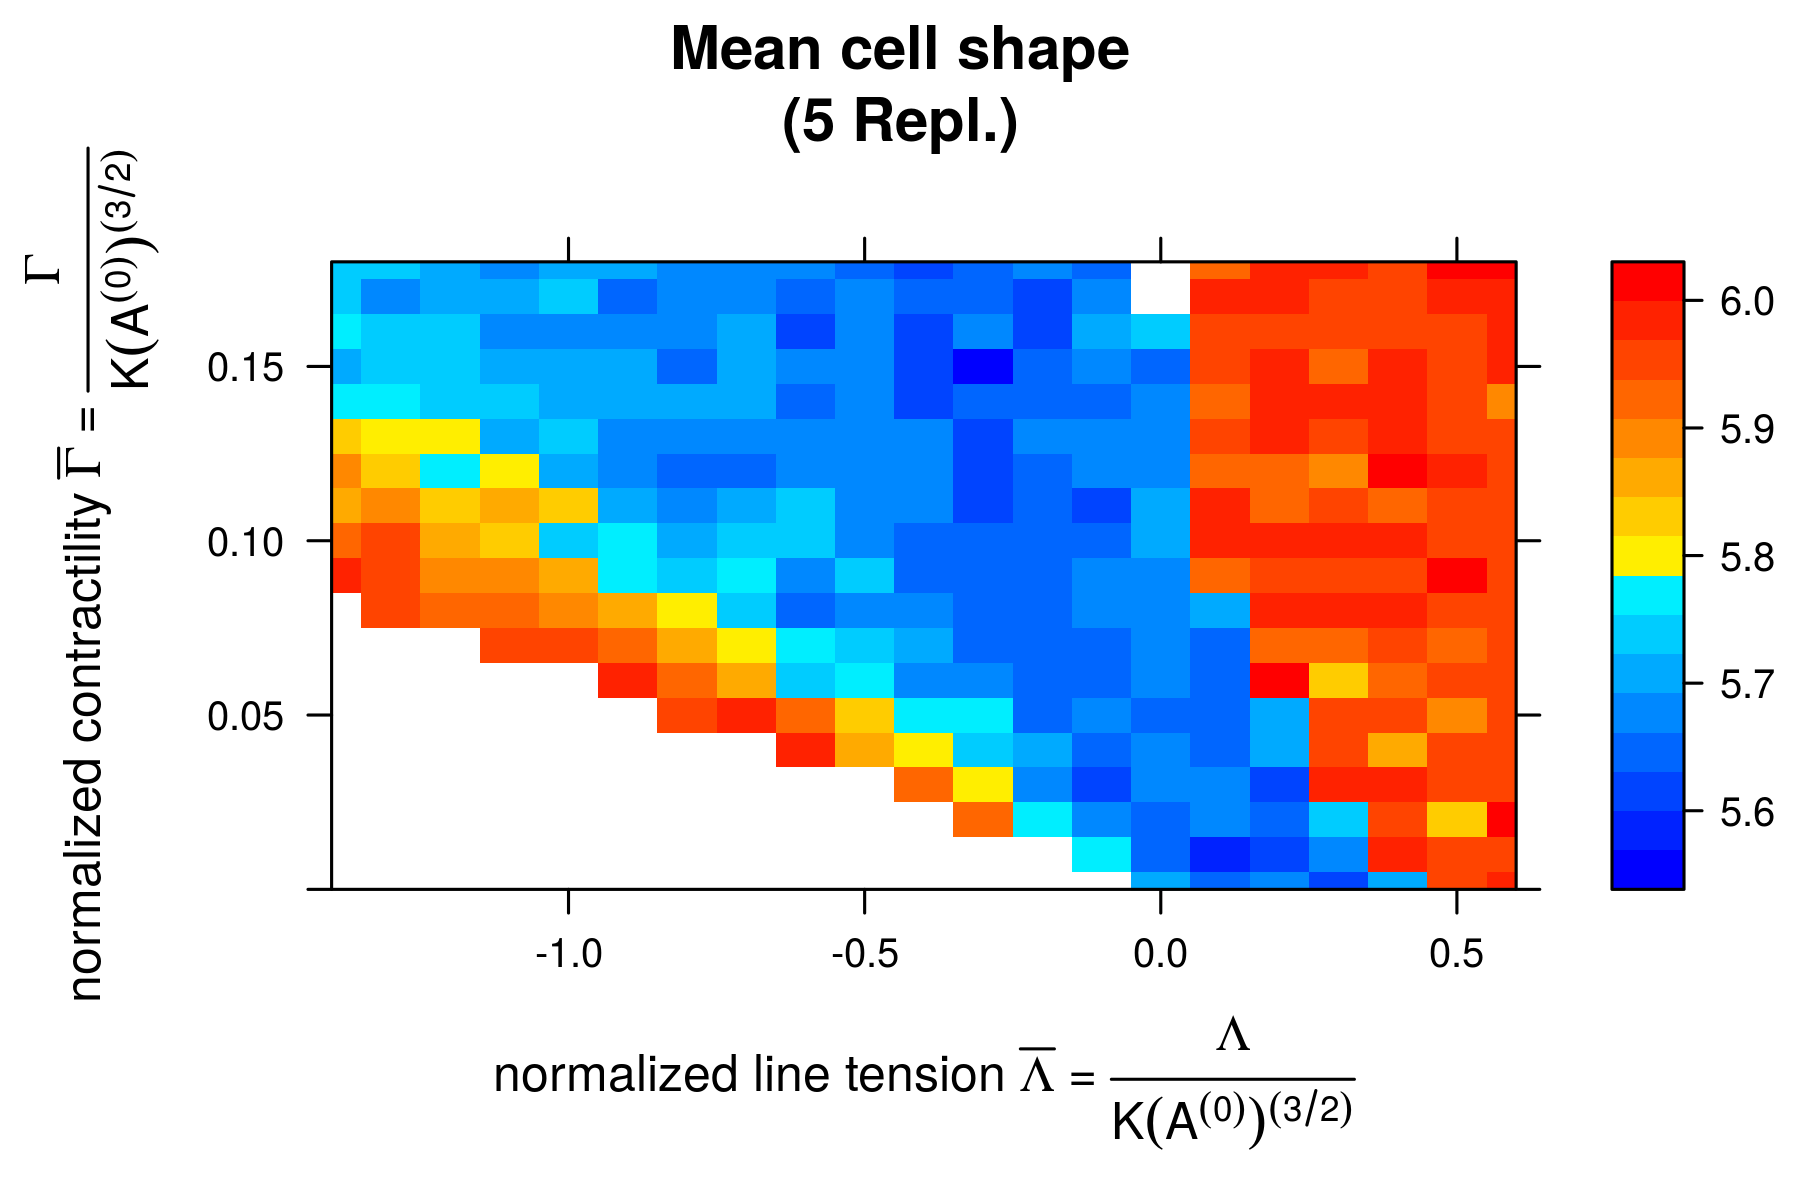
\includegraphics[width=10cm]{levelplot_mean_cellshape.png}
\end{beamerboxesrounded}
}


%%tissue growth remarks
\frame{\frametitle{Phase space: Std. Dev. of shape of cells (5 Repl.)}
\setbeamercolor{uppercol}{fg=black,bg=pink}
\setbeamercolor{lowercol}{fg=black,bg=pink}
\begin{beamerboxesrounded}[upper=upperco,lower=lowercol,shadow=true]{}
\centering \hspace{4cm} 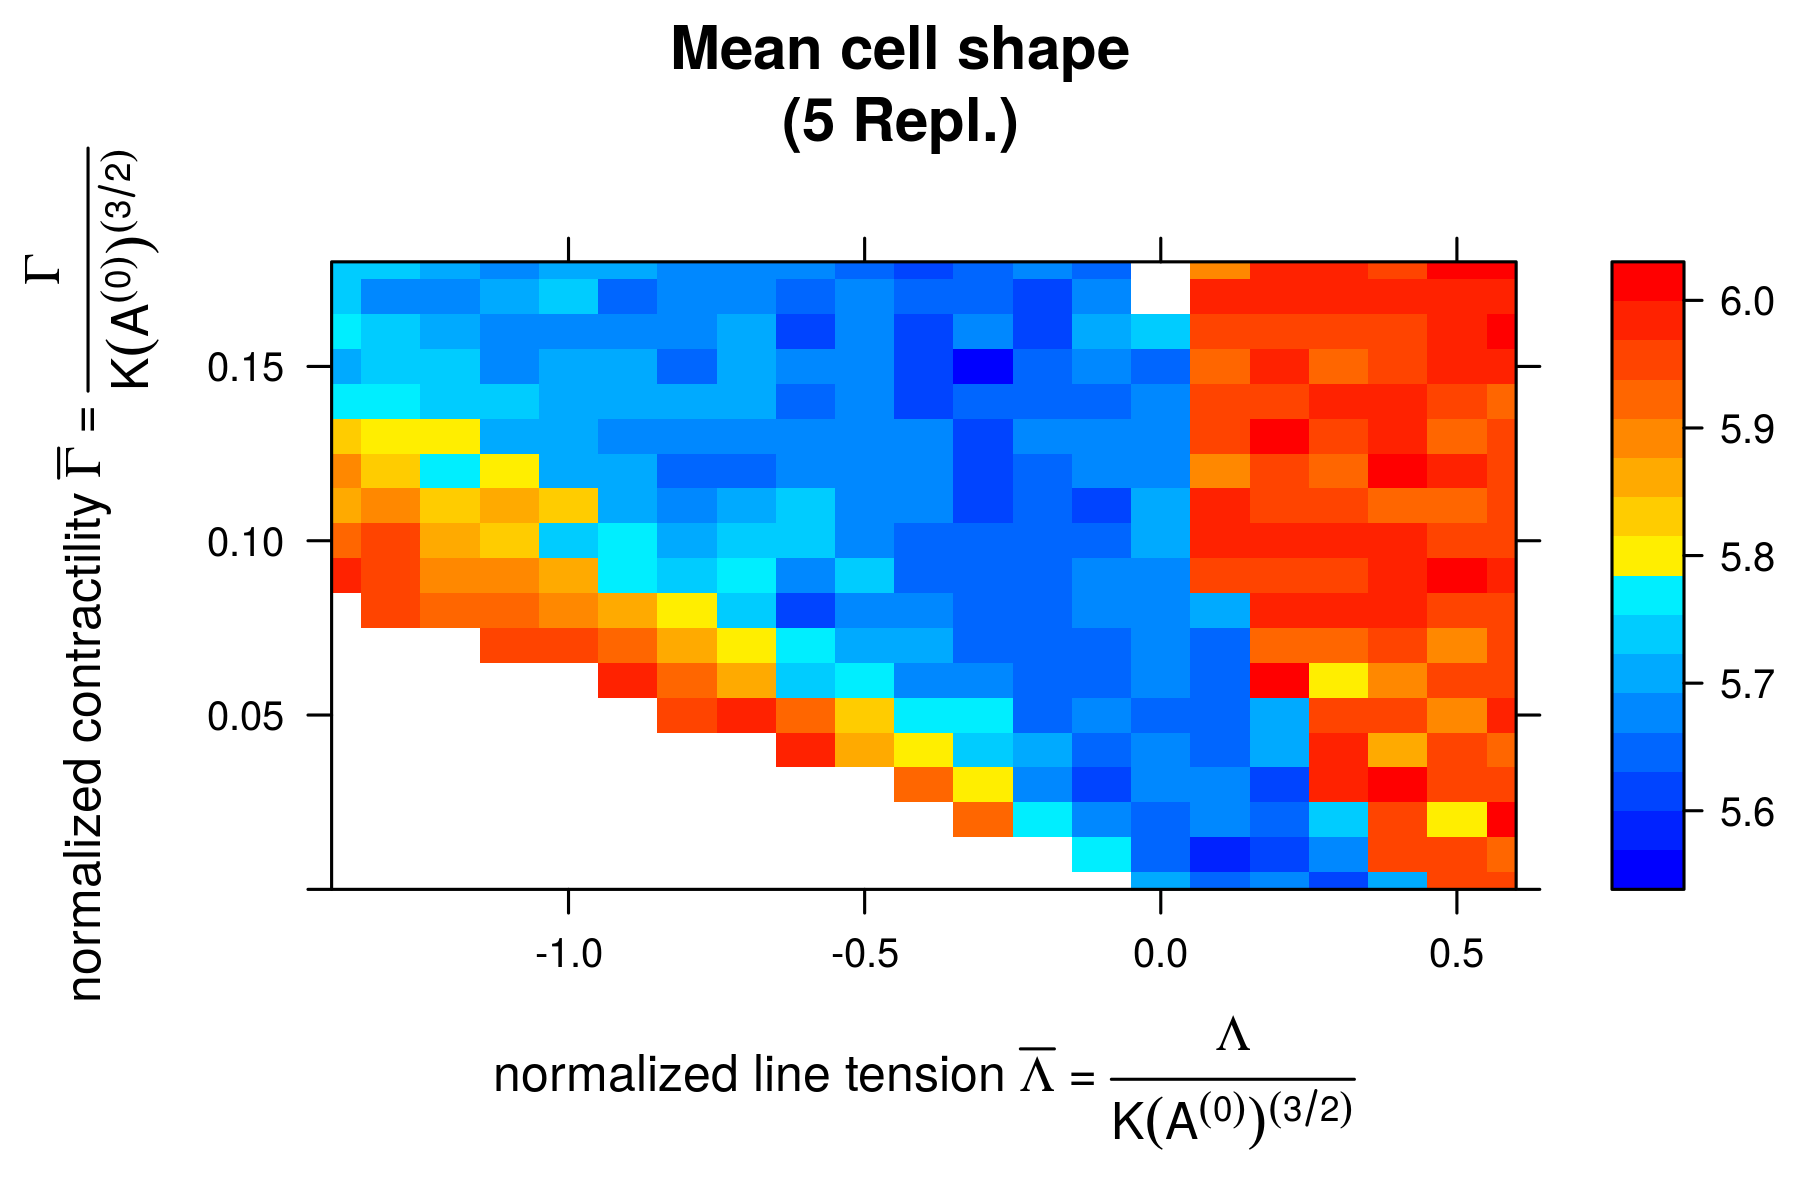
\includegraphics[width=10cm]{levelplot_stdev_cellshape.png}
\end{beamerboxesrounded}
}

%\frame{\frametitle{Phase Space: Deviation of shapes of cells}
%\setbeamercolor{uppercol}{fg=black,bg=pink}
%\setbeamercolor{lowercol}{fg=black,bg=pink}
%\begin{beamerboxesrounded}[upper=upperco,lower=lowercol,shadow=true]{}
%\begin{minipage}[t]{6.1cm}
%\begin{columns}
%    \begin{column}{\textwidth}
%        \hspace{0.4cm} 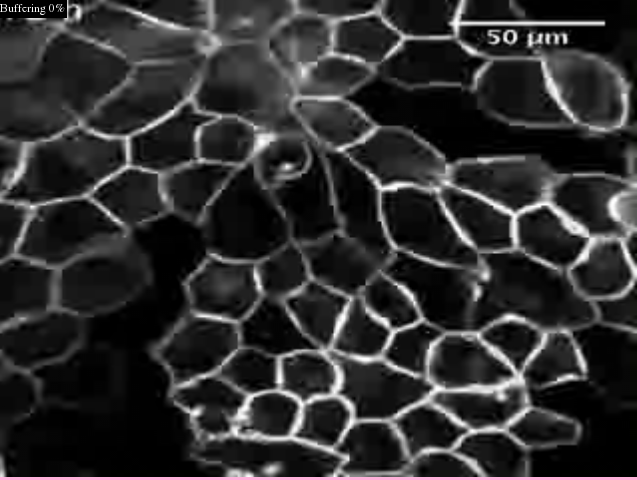
\includegraphics[height=4cm,width=4cm]{network_of_cells.png}
%    \end{column}
%    \begin{column}{0.8\textwidth}
%        \begin{enumerate}
%        \item < 1-| alert@1 > We observed the following Phase space of the variation in the shape of cells after 10 replicates.
%        \end{enumerate}
%    \end{column}
%\end{columns}
%\end{minipage}
%\end{beamerboxesrounded}
%}

\section{Infos}
\subsection{Numbers}
%%tissue growth remarks
\frame{\frametitle{Interesting numbers}
\setbeamercolor{uppercol}{fg=black,bg=pink}
\setbeamercolor{lowercol}{fg=black,bg=pink}
\begin{beamerboxesrounded}[upper=upperco,lower=lowercol,shadow=true]{}
\begin{minipage}[t]{10cm}
    \begin{enumerate}
    \item < 1-| alert@1 > Time to run 5 replicates: \textbf{5 days}
    \item < 2-| alert@2 > Time to run 5 replicates: $9.25 \times 10^{-13}$ AOU.
    \item < 3-| alert@3 > 62k lines of code in \textbf{C++}.
    \item < 4-| alert@4 > Being implemented since 220 days ago.
    \item < 5-| alert@5 > Written by \emph{6 hands}: Aziza Merzouki, Orestis Malaspina, Charles de Santana.
    \end{enumerate}
\end{minipage}
\end{beamerboxesrounded}
}

\subsection{Technologies}
%%tissue growth remarks
\frame{\frametitle{Technologies}
\setbeamercolor{uppercol}{fg=black,bg=pink}
\setbeamercolor{lowercol}{fg=black,bg=pink}
\begin{beamerboxesrounded}[upper=upperco,lower=lowercol,shadow=true]{}
\begin{minipage}[t]{10cm}
    \begin{enumerate}
    \item < 1-| alert@1 > Programming language: \textbf{C++}.
    \item < 2-| alert@2 > Visualization software: \textbf{Paraview} 
    \item < 3-| alert@3 > Statistical analysis and plotting: \textbf{GNU R}
    \item < 4-| alert@4 > Slides made with \textbf{\LaTeX}.
    \end{enumerate}
\end{minipage}
\end{beamerboxesrounded}
}

\section{Future}
\subsection{Very Next Steps}
%%tissue growth remarks
\frame{\frametitle{Very Next steps}
\setbeamercolor{uppercol}{fg=black,bg=pink}
\setbeamercolor{lowercol}{fg=black,bg=pink}
\begin{beamerboxesrounded}[upper=upperco,lower=lowercol,shadow=true]{}
\begin{minipage}[t]{10cm}
    \begin{enumerate}
    \item < 1-| alert@1 > Increase the number of replicates.
    \item < 2-| alert@2 > Explore the parameters at a better \emph{resolution} (varying their values by $10^{-3}$, instead of by $10^{-2}$).
    \item < 3-| alert@3 > Study the Phase Space of Area of cells.
    \item < 4-| alert@4 > Study the Phase Space of \textbf{Area} of cells.
    \item < 5-| alert@5 > Study the Phase Space of \textbf{Perimeter} of cells.
    \item < 6-| alert@6 > Study the Phase Space of \textbf{Direction of edges} of cells.
    \end{enumerate}
\end{minipage}
\end{beamerboxesrounded}
}

\subsection{Next Steps}
%%tissue growth remarks
\frame{\frametitle{Next steps}
\setbeamercolor{uppercol}{fg=black,bg=pink}
\setbeamercolor{lowercol}{fg=black,bg=pink}
\begin{beamerboxesrounded}[upper=upperco,lower=lowercol,shadow=true]{}
\begin{minipage}[t]{10cm}
    \begin{enumerate}
    \item < 1-| alert@1 > Change initial organization of cells in the tissues (starting from non-regular tissues).
    \item < 2-| alert@2 > Change the initial shape of the tissues (starting from ring tissues).
    \item < 3-| alert@3 > Change choice of cells to proliferate (choose the eldest cells with higher probability).
    \item < 4-| alert@4 > Change the way cells are divided (the splitting edge $e_{i}$ depends on the number of edges of neighbour cells).
    \item < 5-| alert@5 > Study 3D tissues.
    \end{enumerate}
\end{minipage}
\end{beamerboxesrounded}
}

\section{Acknowledgments}
\frame{\frametitle{Thank you!}
\begin{itemize}
\item SystemsX Initiative.
\item \textbf{\emph{EpiphysX}} members: Andreas Wagner (UZH), Aziza Merzouki, Orestis Malaspinas, Bastien Chopard, Aur\'elien Roux, Michel Milinkovitch, Marcos Gonzalez-Gaitan, Anastasia Trushko, Antonio Martins (UNIGE) 
\item Chopard's Group members (UNIGE).
\item Wagner's Group members (UZH).
\item You, for the attention and patience.
\end{itemize}
}
%%%%%%%%%%%%%%%%%%%%%%%%%%%%%%%%%%%%%%%%%%%%%%%%%%%%%%%%%%%%%%%%%%%%%%%%%%%%%%%%%%%%%%%%%%
%%%%%%%%%%%%%%%%%%%%%%%%%%%%%% End Document %%%%%%%%%%%%%%%%%%%%%%%%%%%%%%%%%%%%%%%%%%%%%%
%%%%%%%%%%%%%%%%%%%%%%%%%%%%%%%%%%%%%%%%%%%%%%%%%%%%%%%%%%%%%%%%%%%%%%%%%%%%%%%%%%%%%%%%%%
\end{document}


